%% notes-tex/026-kinetics-thermodynamics/026-kinetics-thermodynamics.tex
%% [[experiments.026-metabolism-flux.kinetic-and-thermodynamic-parameter-datasets]]
%% https://github.com/Mjvolk3/torchcell/tree/main/notes-tex/026-kinetics-thermodynamics/026-kinetics-thermodynamics.tex
%%
%% Typeset counterpart of
%% notes/experiments.026-metabolism-flux.kinetic-and-thermodynamic-parameter-datasets.md.
%%
%% Build:  make            -> 026-kinetics-thermodynamics.pdf   (draft: status chips)
%%         make clean-view -> ...-clean.pdf                     (share view)
%%         make check      -> formatting / provenance / style gate
%%         make plots      -> re-convert the matplotlib panels from ASSET_IMAGES_DIR
%%
%% Every number is produced by a committed script under
%% experiments/026-metabolism-flux/scripts/ and read back from
%% experiments/026-metabolism-flux/results/ or from the parquet builds under
%% $DATA_ROOT/data/torchcell/. Nothing here is recalled.

\documentclass[10pt,a4paper]{article}
\usepackage[draft]{tcdoc}
\usepackage{float}
\usepackage{amsmath}
\usepackage{amssymb}

%% Long \texttt paths in prose cannot hyphenate, so give TeX room to stretch a
%% line rather than run it past the text block.
\emergencystretch=3.5em

\title{\vspace{-1.5em}Kinetic and Thermodynamic Parameters\\for the Flux Module\\
  {\large Five predictors run, and formation energies\\
   recomputed with uncertainty}}
\author{Michael Volk}
\date{\today}

\begin{document}
\maketitle
\thispagestyle{empty}

\begin{abstract}
\noindent
The enzyme-constrained flux layer needs three parameter tables and had almost none of
them. Measured $k_{cat}$ covered 148 of 3{,}728 catalytic units, 4.0 percent, with the
other 96 percent running on a single flat default of 10.3 s$^{-1}$; $K_M$ had no table at
all; and the thermodynamics came from a shipped file of point values with no covariance,
usable only for this organism. All three are now built, and every value carries the
\texttt{sha256} of the weights or the model version that produced it.

Six kinetic predictors were mirrored into a standard location with per-file hashes,
retrieval commands and git commits, and five were run over the enzyme-substrate pairs of
yeast-GEM 9.0.2, with protein sequences taken from the genome object rather than from the
table the model bundles. Validating each against its own authors' published examples paid
for itself: \textbf{two of these models exponentiate base 2 and two base 10}, and reading
either wrong yields turnover numbers that still look credible. Two entries in an earlier
readiness audit were reversed by reading files rather than filenames, in both directions,
and a third blocker dissolved entirely once its dependency was checked.

The five predictors agree on the median $k_{cat}$ and disagree per pair. On identical
enzyme-substrate pairs their rank correlation ranges from \textbf{0.015 to 0.509}, with a
typical disagreement of 0.4 to 0.7 decades. Since almost none of these pairs has a measured
value, that spread, and not any published accuracy figure, is the honest uncertainty on a
single predicted turnover number.

Formation energies were recomputed from eQuilibrator's component contribution, which
returns a covariance and applies to any organism because it works from structure. Summing
the resulting table reproduces eQuilibrator's own reaction call to
$9.1\times10^{-13}$ kJ\,mol$^{-1}$, so the table is correct; on the chemical reactions both
tables cover it agrees with the shipped file to a median of 10.11 kJ\,mol$^{-1}$, which is
about as well as the shipped file agrees with itself. The gain is 785 reactions with a
real standard error, median 2.30 kJ\,mol$^{-1}$, and the rank-590 covariance factor the
flux layer had recorded as unavailable. The cost is reaction coverage, 42.5 percent against
77.7. Compartment-specific pH is implemented and not trusted: it moves 1{,}309 reactions by
a median 42 kJ\,mol$^{-1}$, which is not credible.

The predictors agree with each other far less than either agrees with its own training
data, and that gap is the honest uncertainty on any single predicted value.
\end{abstract}

\vspace{0.5em}
\tccontents
\clearpage

%% notes-tex/026-kinetics-thermodynamics/sections/1-mirrors.tex
%% [[experiments.026-metabolism-flux.kinetic-and-thermodynamic-parameter-datasets]]
%% https://github.com/Mjvolk3/torchcell/tree/main/notes-tex/026-kinetics-thermodynamics/sections/1-mirrors.tex

\section{Where the parameters were, and where they are now\secstatus{todo}}
\label{sec:mirrors}

\subsection{The starting state\secstatus{todo}}

Before this work, yeast-GEM 9.0.2 had 3{,}728 catalytic units and one turnover number for
almost none of them. Measured $k_{cat}$ covered 148 units, 4.0 percent, drawn from the Open
Enzyme Database's 1{,}126 \emph{S. cerevisiae} rows, which between them name only 106
distinct UniProt accessions. The other 3{,}580 units, 96 percent of the model, ran on a
single flat default of 10.3 s$^{-1}$, the median of the values that did resolve. $K_M$ had
no table at all: the parameter existed as an enum member and a protocol flag with nothing
behind either.

Thermodynamics was in better shape and worse than it looked, which
Section~\ref{sec:thermo} takes up.

\subsection{A standard place for a model, with provenance\secstatus{todo}}

The predictors arrived as ad-hoc git clones in a scratch directory, which is not something
a result can be rebuilt from: nothing recorded which commit was cloned, and nothing would
detect an upstream force-push. They now live at
\texttt{\$DATA\_ROOT/models/kinetics/<name>/}, beside the existing \texttt{mineru} mirror,
each with a \texttt{manifest.json} pinning every file by \texttt{sha256} and recording the
source URL, the exact retrieval command, and the git commit.

Two trees are kept deliberately apart. \texttt{\$DATA\_ROOT/models/\ldots} holds
\emph{the model}: weights, vocabularies, dictionaries, written once and verified
thereafter. \texttt{\$DATA\_ROOT/data/torchcell/\ldots} holds \emph{what the model
produced}, regenerable from a mirror plus code, and every row carries the
\texttt{sha256} of the weight file that produced it. Deleting a build is routine; deleting
a mirror invalidates the provenance of every build made from it, so a mirror is only ever
added.

The reason to pay this cost is that a predicted $k_{cat}$ is a model output, not a
measurement, and the difference has to survive into the table. A value with no provenance
becomes indistinguishable from a measured one within two steps, and the flux layer's
coverage gate has to tell an experimental value, a predicted value and a filled default
apart.

\subsection{Two corrections to the readiness audit\secstatus{todo}}

An earlier audit of these six repositories recorded which ship weights. Reading the files
rather than the filenames reversed two of its entries, and both reversals matter.

\textbf{DLKcat does ship its trained model.} It is
\texttt{Results/output/all-\/-radius2-\/-\ldots-\/-iteration50}, a PyTorch
\texttt{state\_dict} with no file extension, which is why a scan for
\texttt{*.pt}/\texttt{*.pkl} missed it. On the strength of that miss an 18 GB Zenodo
download had been queued that was never needed.

\textbf{Boost\_KM ships two fitted models, and the citation points at the wrong one.} Its
18 ``weight'' files are the UniRep 1900 mLSTM \emph{featurizer}, and reading only those
supports the conclusion that no regressor was released. Beside them sit
\texttt{xgboost\_model.dat} and \texttt{xgboost\_model\_full.dat}, which are the fitted
$K_M$ regressors, and the repository's own README says the pretrained weights can be
loaded rather than retrained. Nothing needed refitting.

What Wu et al. ran is a third model again. Their Methods cite
\texttt{AlexanderKroll/KM\_prediction}, the repository for the published paper, but the
notebook in their release vendors \texttt{KM\_prediction\_function}, whose enzyme
representation is ESM-1b rather than UniRep and whose regressor,
\texttt{xgboost\_model\_new\_KM\_esm1b.dat}, takes 1{,}332 features rather than 1{,}952.
Kroll's README states the substitution plainly: ``the model provided in the repository
`KM\_prediction\_function' is slighly different to the one presented in our paper: Instead
of the UniRep model, we are using the ESM-1b model.'' The substrate encoder is common to
both, and its three checkpoint files are byte-identical across the two repositories, so
only the enzyme half and the regressor differ. Reproducing Fig.~3f means following the
code rather than the citation.

\subsection{One environment per predictor\secstatus{todo}}

A released predictor is a frozen artifact, and several of them pin dependencies that cannot
coexist. UniKP's regressors were pickled before scikit-learn 1.3 added
\texttt{missing\_go\_to\_left} to the decision-tree node dtype, and scikit-learn 1.7
refuses to load them. Refusing is correct: reinterpreting a tree's node array under a
changed dtype would yield numbers that are not UniKP's predictions.

So UniKP runs in an environment pinned to scikit-learn 1.2.2, invoked as a subprocess with
parquet as the interface, and the torchcell-side dataset class calls it rather than
importing it. Treating that as an accident to be patched around would be a mistake; it is
the shape this has to take, and DeepEnzyme additionally wants NVIDIA apex and an old numpy
for the same reason.

%% notes-tex/026-kinetics-thermodynamics/sections/2-predictors.tex
%% [[experiments.026-metabolism-flux.kinetic-and-thermodynamic-parameter-datasets]]
%% https://github.com/Mjvolk3/torchcell/tree/main/notes-tex/026-kinetics-thermodynamics/sections/2-predictors.tex

\section{The predictors, and what running them taught\secstatus{todo}}

\subsection{One module per model, on the node-embedding pattern\secstatus{todo}}

Which predictor feeds the flux layer is a design choice to experiment over, not a pipeline
detail to settle once, so the kinetic predictors copy the shape the sequence-embedding
datasets already use: an abstract base, one module per model, and a name-to-class registry
that a config string selects.

One structural difference drives everything else. A node embedding is keyed by
\emph{gene}; a kinetic parameter is keyed by a \emph{pair}, because a turnover number is a
property of one enzyme acting on one substrate. The key is
$(\textrm{uniprot}, \textrm{substrate}, \textrm{predictor}, \textrm{parameter})$.
Collapsing to one row per gene would silently pick a substrate, and collapsing to one row
per catalytic unit would silently pick a subunit, so the store holds pairs and aggregation
lives in the resolver. The dataset records what was predicted; the caller decides what the
layer sees.

\subsection{Sequences come from the genome, not from the model's bundled table\secstatus{todo}}

yeast-GEM ships a \texttt{swissprot.tsv} with a sequence column, and it sits conveniently
beside the model. It is the wrong source. Protein sequences are read from
\texttt{SCerevisiaeGenome} through \texttt{genome[orf].protein.seq}, the same path the ESM2
embedding dataset uses, so everything stays on the derivation chain from the S288C
reference FASTA plus the GAF. The difference is provenance rather than content: a sequence
from a third-party table is a claim by that table's compiler, while the same sequence from
the genome is the one the perturbation ontology edits, so a strain's genotype and the
protein a predictor sees cannot silently disagree.

All 1{,}161 yeast-GEM genes resolve as \texttt{current} through the shared gene-name
reconciler, and all 1{,}161 have a protein sequence, so nothing is lost by the switch.
Rebuilding DLKcat on genome sequences moved the median $k_{cat}$ from 4.0125 to 4.0116
s$^{-1}$, which says the two sources agree on content and differ on provenance.

Two failures are worth recording because both are silent. \texttt{orf in genome} looks
safer than indexing and is not: the genome defines no \texttt{\_\_contains\_\_}, so Python
falls back to integer indexing and calls \texttt{genome[0]}, raising before the real lookup
happens. And \texttt{go\_root} is a separate constructor argument defaulting to a relative
path; left unset it misses and the constructor tries to fetch \texttt{go.obo} from
\texttt{current.geneontology.org}, which answers 403.

\subsection{Validation caught a log base\secstatus{todo}}

The DLKcat implementation reproduces the authors' three released example values to four
decimal places. That check was worth more than its cost, because it caught two defects that
would otherwise have been invisible in a plausible-looking table.

\textbf{The output is $\log_2$, not $\log_{10}$.} The authors exponentiate with
\texttt{math.pow(2, \ldots)}. Reading it as base 10 inflates every turnover number by a
power of roughly 3.3 and still produces numbers that look like credible turnover numbers.

\textbf{Multi-component SMILES are refused by the model itself.} Its fingerprint pass
indexes a node list built only from bonded atoms, so a disconnected fragment, such as the
lone \texttt{[Fe+2]} in the heme SMILES yeast-GEM gives for ferricytochrome $c$, walks off
the end of the list. Excluding them is what the model does, so the exclusion is recorded
rather than worked around.

\subsection{Embedding on four GPUs\secstatus{todo}}

UniKP's protein half is ProtT5-XL, a 3-billion-parameter encoder, and its pinned
environment holds CPU-only torch. The embedding is therefore produced once on GPU and
handed across as a content-addressed cache, keyed by a hash of the sequence so that any
predictor wanting a ProtT5 representation can reuse it and two ORFs with one sequence
resolve to one vector.

Sequences are split by index across the four GPUs and merged; within a shard they are
sorted by length and batched, which is where most of the gain comes from, and a
per-sequence masked mean keeps the result identical to unbatched inference. The 1{,}154
distinct sequences finish in under 40 seconds.

The genome is read exactly once, by a dump step, and the shards read that dump. Four
processes opening the same gffutils SQLite database concurrently raced and made it briefly
unreadable; since the shards need the genome for nothing but a sequence lookup, the
dependency was removed rather than serialized.

\subsection{What each predictor cost to run\secstatus{todo}}

%% SOURCE: hand-authored from the mirror manifests written by
%% experiments/026-metabolism-flux/scripts/mirror_kinetic_models.py; the machine
%% readable form is experiments/026-metabolism-flux/results/kinetic_model_mirrors.json
\begin{table}[H]
  \centering
  \footnotesize
  \caption[Predictor status]{The six predictors named in Wu et al.'s Methods, what each
  emits, and what it took to run here. ``Ships weights'' refers to the repository as
  cloned; UniKP's fitted regressors are released separately on HuggingFace and are
  mirrored alongside it.}
  \label{tab:predictors}
  \begin{tabular}{llll}
    \hline
    Predictor & Emits & Ships weights & Note \\
    \hline
    DLKcat & $k_{cat}$ & yes, extensionless & output is $\log_2$ \\
    UniKP & $k_{cat}$, $K_M$ & regressors on HuggingFace & needs scikit-learn 1.2.2 \\
    TurNuP & $k_{cat}$ & Zenodo archive & takes full reaction SMILES \\
    EITLEM-Kinetics & $k_{cat}$, $K_M$ & Zenodo, 12.3 GB & many checkpoints \\
    Boost\_KM & $K_M$ & yes, two regressors & ESM-1b variant is the one Wu ran \\
    DeepEnzyme & $k_{cat}$ & figshare & uses AlphaFold structures \\
    \hline
  \end{tabular}
\end{table}

%% notes-tex/026-kinetics-thermodynamics/sections/3-thermodynamics.tex
%% [[experiments.026-metabolism-flux.kinetic-and-thermodynamic-parameter-datasets]]
%% https://github.com/Mjvolk3/torchcell/tree/main/notes-tex/026-kinetics-thermodynamics/sections/3-thermodynamics.tex

\section{Thermodynamics recomputed from eQuilibrator\secstatus{todo}}
\label{sec:thermo}

\subsection{Why the shipped table is a dead end\secstatus{todo}}

yeast-GEM 9.0.2 ships \texttt{model\_metDeltaG.csv} and \texttt{model\_rxnDeltaG.csv}, and
they are usable: 2{,}389 of 2{,}806 metabolites and 3{,}210 of 4{,}131 reactions carry a
value. They also close two doors. They are point values with no covariance, so the
correlated error term $\Delta_r G^{\circ,\mathrm{error}} = Qm$ that a thermodynamic flux
formulation calls for cannot be formed from them at all. And they exist only for this
model, so a table built on them transfers to no other organism.

Component contribution answers both at once. It decomposes a compound into groups, fits
group energies against the measured reaction corpus, and returns a formation energy
together with the covariance implied by that fit. Applied to a structure it works for any
organism, and for compounds no database has tabulated.

Reading the shipped files correctly is itself a trap worth recording. They use
\emph{two} missing-value conventions: most gaps are the sentinel $10^7$, but a further 51
metabolites and 120 reactions are the literal string \texttt{NaN}. Filtering only the
sentinel leaves the NaNs, which then propagate through every sum and produce NaN gradients
from what looks like a coverage of 87 percent.

\subsection{Resolution, and what it costs\secstatus{todo}}

Each metabolite is resolved by accession, MetaNetX first, then ChEBI, then KEGG, then
BiGG, with an InChI structure lookup as a fallback. Figure~\ref{fig:thermo-resolution}
shows where they land: MetaNetX carries almost all of it, and 332 metabolites resolve to
nothing.

\begin{figure}[H]
  \centering
  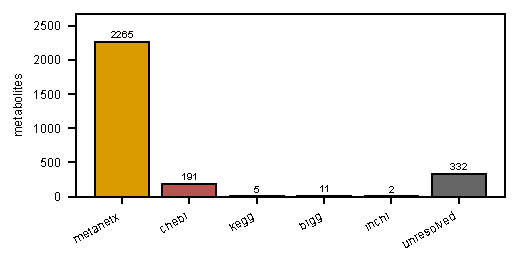
\includegraphics[width=0.62\textwidth]{figures/thermo_a_resolution.pdf}
  \caption[Metabolite resolution by identifier namespace]{Which identifier namespace
  resolved each of yeast-GEM's 2{,}806 metabolites to an eQuilibrator compound, in the
  order the resolver tries them. A metabolite counted under \texttt{chebi} is one whose
  MetaNetX identifier missed, so the bars are disjoint rather than nested. The 332
  unresolved are dominated by acyl-CoA isomers and the \texttt{biomass} pseudo-metabolite.
  Generated by \texttt{experiments/026-metabolism-flux/scripts/plot\_equilibrator\_thermo.py}.}
  \label{fig:thermo-resolution}
\end{figure}

The coverage cost is real and is stated rather than softened. Against the shipped table's
2{,}389 metabolites and 3{,}210 reactions, the recomputation covers 2{,}099 metabolites
(74.8 percent) and 1{,}755 reactions with every participant known (42.5 percent). Buying
uncertainty and organism-independence costs reaction coverage, because a reaction needs
\emph{all} of its participants resolved before it has an energy at all.

\subsection{The uncertainty, which is the point\secstatus{todo}}

Figure~\ref{fig:thermo-uncertainty} shows the standard error on the reactions whose energy
is estimable. Two facts sit inside it. Of 1{,}673 estimable reactions, 888 have a standard
error of exactly zero; those are transport reactions, where the same compound appears on
both sides of the membrane and its uncertainty cancels term by term. The remaining 785
carry a genuine standard error with a median of 2.30 kJ\,mol$^{-1}$ and a 95th percentile
of 6.01.

Estimability is a separate question from uncertainty and is easy to conflate. Component
contribution returns two sets of directions, one with finite variance and one with
infinite variance, the latter being directions the training corpus never determined.
Almost every individual compound has a nonzero infinite component, because an absolute
formation energy is defined only up to element conservation. Those directions cancel in a
mass-balanced reaction, which is exactly why the test must be applied to a reaction and
never to a compound in isolation. A reaction whose infinite component does not cancel has
an energy that is undefined rather than uncertain, and reporting it with a finite error bar
would be the most misleading thing this table could do, so it is masked instead.

\begin{figure}[H]
  \centering
  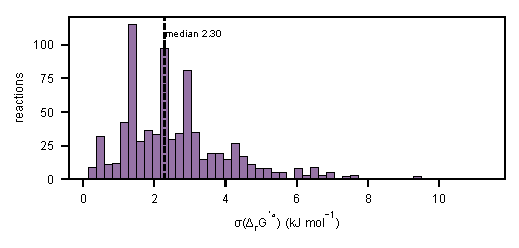
\includegraphics[width=0.62\textwidth]{figures/thermo_c_uncertainty.pdf}
  \caption[Reaction standard error from component contribution]{Standard error on
  $\Delta_r G'^\circ$ for the 785 estimable reactions whose uncertainty is nonzero, with
  the median marked. The 888 estimable reactions omitted here have a standard error of
  exactly zero because they are transport steps whose per-compound uncertainties cancel.
  The shipped table carries no uncertainty of any kind, so this quantity has no
  counterpart in it. Generated by
  \texttt{experiments/026-metabolism-flux/scripts/plot\_equilibrator\_thermo.py}.}
  \label{fig:thermo-uncertainty}
\end{figure}

\subsection{Agreement with the shipped table\secstatus{todo}}

Figure~\ref{fig:thermo-vs-shipped} compares the two tables on the 1{,}391 reactions both
cover, at a uniform pH 7.0 so that the comparison is between methods rather than between
pH assumptions.

The two classes of reaction must be read separately, and pooling them produces a
misleadingly good number. At a single uniform pH a transport reaction moves a species
between compartments with the same formation energy on both sides, so its energy here is
exactly zero by construction while the shipped table carries a nonzero value for it. Those
840 reactions form the horizontal band at zero. On the 551 chemical reactions, which is
where the two methods actually make comparable claims, the median absolute difference is
\textbf{10.11 kJ\,mol$^{-1}$}. Pooling all 1{,}391 gives 5.60, and that smaller number is
an artifact of the transport band rather than better agreement.

For scale, the shipped table disagrees with \emph{itself} by a comparable amount: the
reaction file and the reaction energies recomputed from its own metabolite file differ by a
median of 9.53 kJ\,mol$^{-1}$. So the two methods agree about as well as the shipped table
is internally consistent, which is the honest reading.

\begin{figure}[H]
  \centering
  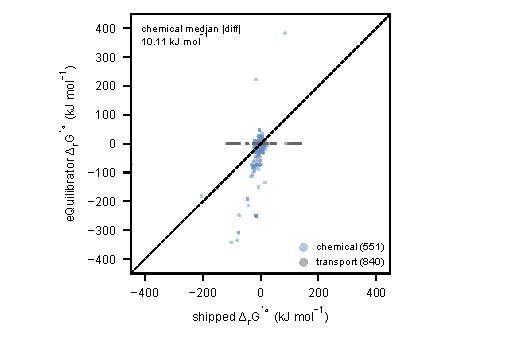
\includegraphics[width=0.62\textwidth]{figures/thermo_d_vs_shipped.pdf}
  \caption[eQuilibrator against the shipped reaction energies]{Reaction energies from the
  recomputation against the values yeast-GEM ships, on the 1{,}391 reactions both cover, at
  uniform pH 7.0, ionic strength 0.25 M and 303.15 K. Chemical reactions and transport
  reactions are separated because a transport step is exactly zero here by construction:
  at one pH the same species has the same formation energy in both compartments. The
  quoted median absolute difference is for the chemical subset. The dashed line is
  equality. Generated by
  \texttt{experiments/026-metabolism-flux/scripts/plot\_equilibrator\_thermo.py}.}
  \label{fig:thermo-vs-shipped}
\end{figure}

\subsection{Compartment pH is implemented and not trusted\secstatus{todo}}

Applying a per-compartment pH rather than a uniform one moves 1{,}309 of 1{,}755 covered
reactions, by a median of 42.2 kJ\,mol$^{-1}$ and by as much as 1{,}062
(Figure~\ref{fig:thermo-ph}). Shifts of that size are not physically plausible for single
reactions, so the uniform build is the artifact to use and the compartment build is
experimental. The pH table itself is textbook organellar values, recorded in the output as
\texttt{assumed}, not sourced from a mirrored paper.

The motivation for wanting it remains: a proton crossing a membrane between two pH values
is the entire driving force of a transport step, and computing every compartment at one pH
sets that force to zero by construction. Diagnosing the oversized shifts is open work.

\begin{figure}[H]
  \centering
  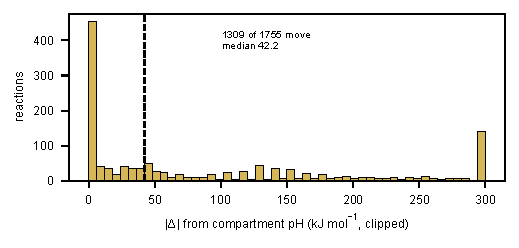
\includegraphics[width=0.62\textwidth]{figures/thermo_e_compartment_ph.pdf}
  \caption[Effect of compartment-specific pH]{Absolute change in $\Delta_r G'^\circ$ when
  each metabolite is transformed at its compartment's pH rather than at a uniform 7.0,
  over the reactions covered in both builds, clipped at 300 kJ\,mol$^{-1}$ for display.
  The median shift of 42.2 kJ\,mol$^{-1}$ is too large to be credible for ordinary
  reactions, which is why the uniform build is preferred. Generated by
  \texttt{experiments/026-metabolism-flux/scripts/plot\_equilibrator\_thermo.py}.}
  \label{fig:thermo-ph}
\end{figure}

\subsection{The correctness check\secstatus{todo}}

The table stores per-metabolite formation energies because that is what the flux layer
consumes, and reaction energies follow as $\sum_i S_{ij}\Delta_f G'^\circ_i$. That identity
is an assumption until tested: an error in the Legendre transform, in the compartment pH
assignment, or in a stoichiometric sign would each produce a table that looks entirely
reasonable and is wrong.

Pricing the same reactions both ways, by summing the table and by handing the resolved
compounds to eQuilibrator's own \texttt{standard\_dg\_prime}, agrees to a maximum absolute
difference of $9.1\times10^{-13}$ kJ\,mol$^{-1}$ over 40 single-compartment mass-balanced
reactions (Figure~\ref{fig:thermo-validation}). Only single-compartment reactions are used,
because a reaction spanning two compartments has no single pH and the API call would not be
answering the same question; only balanced ones, because an unbalanced reaction carries an
arbitrary offset.

As an absolute check that eQuilibrator is configured correctly before anything is compared
against it, four textbook reactions price at pH 7.2, ionic strength 0.25 M and 303.15 K as:
ATP hydrolysis $-28.93 \pm 0.30$, phosphoglucose isomerase $+2.66 \pm 0.38$, fumarase
$-3.43 \pm 0.28$ and triosephosphate isomerase $+5.61 \pm 0.55$ kJ\,mol$^{-1}$.

\begin{figure}[H]
  \centering
  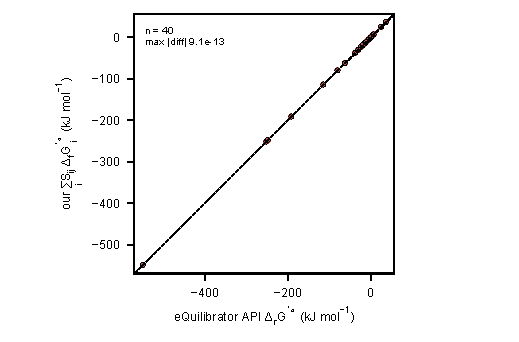
\includegraphics[width=0.62\textwidth]{figures/thermo_f_validation.pdf}
  \caption[Sum of formation energies against the eQuilibrator reaction call]{Reaction
  energies computed by summing our per-metabolite table against the same reactions priced
  directly by eQuilibrator's \texttt{standard\_dg\_prime}, over 40 randomly chosen
  single-compartment mass-balanced reactions. Maximum absolute difference
  $9.1\times10^{-13}$ kJ\,mol$^{-1}$, which is floating-point noise. This is a correctness
  check rather than a result: had the points left the diagonal, nothing else in this
  section would mean anything. Generated by
  \texttt{experiments/026-metabolism-flux/scripts/validate\_equilibrator\_thermo.py} and
  \texttt{plot\_equilibrator\_thermo.py}.}
  \label{fig:thermo-validation}
\end{figure}

\subsection{Where the method stops\secstatus{todo}}

The betaxanthin cassette is the test of the claim that this transfers to compounds no
database has tabulated. Of five intermediates, all five match their declared molecular
formula against a PubChem structure lookup, and two resolve to a formation energy:
L-DOPA at $-157.68$ with $\sigma = 4.30$, and dopaquinone at $-168.31$ with $\sigma = 7.54$
kJ\,mol$^{-1}$, both from structure alone with no identifier required.

The other three, cyclo-DOPA, betanidin and betalamic acid, are absent from the compound
cache, and the blocker is a \emph{commercial license rather than a method}. Creating a new
compound runs a group decomposition that needs pKa estimates, and eQuilibrator obtains
those from ChemAxon's \texttt{cxcalc}; without that license
\texttt{equilibrator\_assets} loads in read-only mode and refuses to create compounds. So
the generalization claim holds for structures the cache already knows and fails for
genuinely new ones. Closing the gap needs a pKa route that does not pass through ChemAxon,
not more plumbing.

%% notes-tex/026-kinetics-thermodynamics/sections/4-reproduction.tex
%% [[experiments.026-metabolism-flux.scripts.plot_kinetic_distributions]]
%% https://github.com/Mjvolk3/torchcell/tree/main/notes-tex/026-kinetics-thermodynamics/sections/4-reproduction.tex

\section{Reproducing Wu et al.'s Fig.~3\secstatus{todo}}

\subsection{What the original figure claims\secstatus{todo}}

Wu et al. (2026) build Yeast-MetaTwin, a comprehensive metabolic network for
\emph{S.~cerevisiae} obtained by expanding reaction rules over the yeast metabolome, and
ask how the resulting \emph{underground} reactions differ kinetically from the
\emph{core} network already in Yeast9. Their Fig.~3a--h answers it with eight empirical
cumulative distributions, one per predictor and parameter: $k_{cat}$ from DLKcat, UniKP,
EITLEM-Kinetics, TurNuP and DeepEnzyme, then $K_M$ from Boost\_KM, UniKP and
EITLEM-Kinetics. Their conclusion is that underground metabolism is separated from known
metabolism by $K_M$ rather than by $k_{cat}$.

The construction is taken from their own notebook: sort the values, plot the running
proportion, and mark each curve's median with a short vertical tick. Their split is on
whether a reaction identifier contains \texttt{rxn}, which is how their tables encode a
predicted rather than a curated reaction.

\subsection{The per-pair predictions behind Fig.~3 were not released\secstatus{todo}}

The intention was to draw two things on each panel: the authors' own released predictions
split core against underground, and our independent re-run over yeast-GEM. The first is not
available.

Their notebook reads its tables from \texttt{Results/kcat\_km\_predict/}, naming each one
explicitly:

\begin{itemize}\setlength{\itemsep}{0pt}
  \item \texttt{yeast8U\_kcat\_predict.csv} \quad DLKcat
  \item \texttt{yeast8U\_unikp.csv} \quad UniKP, both parameters
  \item \texttt{yeast8U\_kcat\_result\_TurNuP.csv} \quad TurNuP
  \item \texttt{yeast8U\_km\_km\_predict.csv} \quad Boost\_KM
\end{itemize}

\noindent That directory is in neither released artifact. The GitHub repository ships \texttt{Results/} with nine subdirectories, none of
them \texttt{kcat\_km\_predict}, and its \texttt{source\_data} holds only
\texttt{fig2-a}, \texttt{fig3-g}, \texttt{fig3-j}, \texttt{fig4-b}, \texttt{fig5-b},
\texttt{figs11} and \texttt{figS8}; the file named \texttt{fig3-g.csv} contains EC-number
counts rather than a $K_M$ distribution. The 6.6 GB Zenodo archive
(10.5281/zenodo.13911783) contains exactly three top-level directories, \texttt{Data},
\texttt{Data\_retrosynthesis} and \texttt{esm}, and of its 1{,}021{,}022 entries
\textbf{zero} match \texttt{kcat}, \texttt{unikp}, \texttt{turnup}, \texttt{eitlem} or
\texttt{deepenzyme}.

This is checkable and is stated as a fact about the release rather than as a criticism of
the work: the Data Availability statement says data for reproducing all figures is
available on GitHub and Zenodo, and for Fig.~3a--h it is not.

Two consequences follow. The \textbf{underground arm cannot be drawn}, because generating
the Yeast-MetaTwin reaction set is a separate retrobiosynthesis pipeline that this work
does not rebuild. And what remains is the stronger half of a reproduction anyway: the
curves in Figure~\ref{fig:kinetics-fig3} are re-derived by running the same published
models over the same organism from hash-pinned mirrors, rather than re-plotted from
someone else's numbers.

\begin{figure}[H]
  \centering
  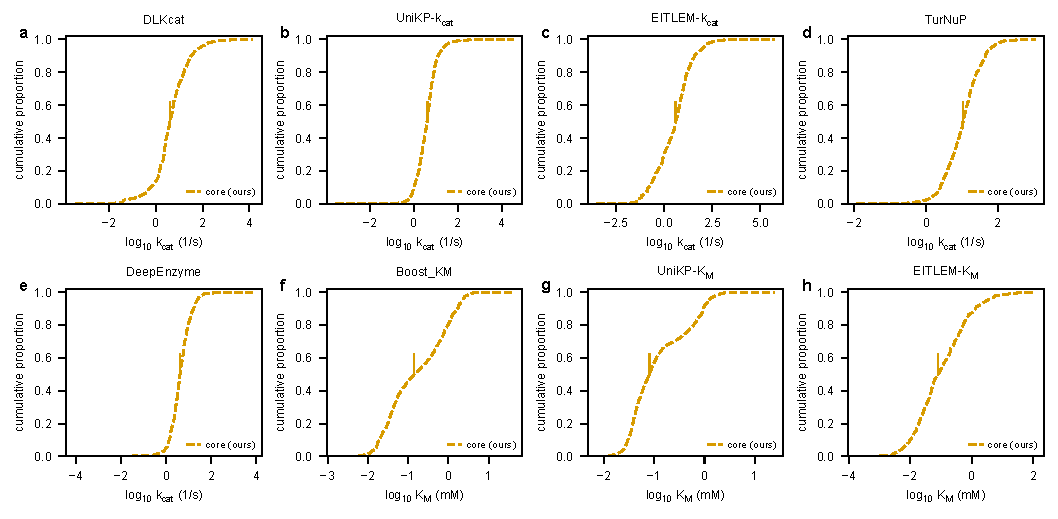
\includegraphics[width=\textwidth]{figures/kinetics_fig3.pdf}
  \caption[Predicted kinetic parameter distributions, after Wu et al. Fig.~3a--h]{Empirical
  cumulative distributions of predicted kinetic parameters, following Wu et al. (2026)
  Fig.~3a--h. Panels a--e are $k_{cat}$, panels f--h are $K_M$; the predictor is named on
  each panel. Amber dashed is our independent run of the same predictor over yeast-GEM
  9.0.2, which is the core network. The authors' core and underground curves are absent
  because the per-pair tables their notebook reads are in neither released artifact, as
  the text sets out. A short vertical tick marks each curve's median, as in the original.
  All eight predictors ran, so every panel carries a curve. Generated
  by
  \texttt{experiments/026-metabolism-flux/scripts/plot\_kinetic\_distributions.py}.}
  \label{fig:kinetics-fig3}
\end{figure}

\subsection{The log base is not a convention\secstatus{todo}}

Each predictor was validated against something its own authors published, and the exercise
paid for itself. \textbf{Two of these models exponentiate base 2 and two base 10}, and
reading either wrong produces turnover numbers that look entirely credible.

\begin{table}[H]
  \centering
  \footnotesize
  \caption[Author-example validation]{What each predictor was checked against before its
  output was believed, and the exponentiation base that check established.}
  \label{tab:validation}
  %% SOURCE: each run's own self-test, reported in the per-predictor summary JSON under
  %% $DATA_ROOT/data/torchcell/kinetics/<predictor>/processed/.
  \begin{tabular}{@{}p{0.16\textwidth}p{0.52\textwidth}l@{}}
    \hline
    Predictor & Checked against & Base \\
    \hline
    DLKcat & 3 released examples, to 4 decimals & $\log_2$ \\
    DeepEnzyme & 137/137 checkpoint tensors match; 3 independent base checks & $\log_2$ \\
    EITLEM & README worked example, 1.3904 vs a stated 1.39 & $\log_{10}$ \\
    TurNuP & tutorial value, 216.114853 vs 216.114853 & $\log_{10}$ \\
    \hline
  \end{tabular}
\end{table}

Two blockers in an earlier audit also dissolved on inspection. DeepEnzyme's NVIDIA apex
requirement is listed in \texttt{requirements.txt} and imported nowhere in its code, so it
was a training-time mixed-precision dependency and the network runs unmodified. TurNuP's
weights exist but are split across two Zenodo records, because the enzyme half needs an
ESM-1b fine-tune that ships only with the prediction-function archive.

\subsection{The comparison between predictors, which the original does not make\secstatus{todo}}

Reading the panels side by side invites a question the paper does not ask: do the
predictors agree with each other? Four of the five agree on the median $k_{cat}$ to within
4.0 to 4.2 s$^{-1}$, and that agreement is superficial. Their \emph{per-pair} rank
correlation, on identical enzyme-substrate pairs, ranges from \textbf{0.015 to 0.509}.

\begin{table}[H]
  \centering
  \footnotesize
  \caption[Predictor agreement]{Agreement between predictors on identical
  enzyme-substrate pairs, in $\log_{10}$ space. The last column is the median absolute
  difference in decades. Produced by
  \texttt{experiments/026-metabolism-flux/scripts/compare\_kinetic\_predictors.py}.}
  \label{tab:agreement}
  %% SOURCE: experiments/026-metabolism-flux/results/kinetic_predictor_comparison.json
  \begin{tabular}{@{}lrrrr@{}}
    \hline
    Pair & $n$ & Pearson & Spearman & Med.\ $|$diff$|$ \\
    \hline
    EITLEM vs UniKP & 7{,}351 & 0.560 & 0.509 & 0.51 \\
    TurNuP vs UniKP & 5{,}038 & 0.458 & 0.433 & 0.44 \\
    EITLEM vs TurNuP & 5{,}143 & 0.361 & 0.330 & 0.64 \\
    DLKcat vs UniKP & 7{,}351 & 0.337 & 0.224 & 0.46 \\
    DeepEnzyme vs DLKcat & 7{,}300 & 0.270 & 0.284 & 0.40 \\
    DLKcat vs EITLEM & 7{,}351 & 0.248 & 0.169 & 0.70 \\
    DLKcat vs TurNuP & 5{,}038 & 0.142 & 0.084 & 0.56 \\
    DeepEnzyme vs TurNuP & 5{,}035 & 0.111 & 0.094 & 0.51 \\
    DeepEnzyme vs UniKP & 7{,}300 & 0.109 & 0.015 & 0.40 \\
    DeepEnzyme vs EITLEM & 7{,}300 & 0.090 & 0.025 & 0.68 \\
    \hline
    $K_M$: Boost\_KM vs UniKP & 7{,}157 & 0.764 & 0.789 & 0.29 \\
    $K_M$: EITLEM vs UniKP & 7{,}351 & 0.463 & 0.406 & 0.50 \\
    $K_M$: Boost\_KM vs EITLEM & 7{,}157 & 0.359 & 0.345 & 0.54 \\
    \hline
  \end{tabular}
\end{table}

That matters for how Fig.~3 should be read. A shift between two curves within one panel is
interpreted as a property of underground metabolism; the spread \emph{between} panels, on
the same pairs, is a factor of three to five. An effect smaller than that sits inside the
disagreement between the instruments measuring it, which is consistent with the paper's own
conclusion being framed on $K_M$, where the separation is large, rather than on $k_{cat}$,
where it is small.

TurNuP is the exception to the median agreement, at 10.8 s$^{-1}$, and its coverage is
55.2 percent rather than 95. Both follow from the same property: it consumes the
\emph{whole reaction}, and the authors' code invalidates a reaction as soon as one
participant lacks a structure. That excludes 1{,}147 of 2{,}540 reactions, almost all
acyl-chain-resolved lipids.

\subsection{The comparison per gene, which is the unit the model reads\secstatus{todo}}

Table~\ref{tab:agreement} is keyed by enzyme-substrate pair. That is the right key for
asking whether two models predict the same number for the same measurement, and it is not
the key the flux layer reads: a catalytic unit draws one $k_{cat}$ per gene. So the
question that decides whether a predicted table is usable is how far the choice of
predictor moves \emph{that gene's} value. Figure~\ref{fig:per-gene} answers it, taking each
gene's value as the median over its pairs in $\log_{10}$ space, separately per predictor.

\begin{figure}[H]
  \centering
  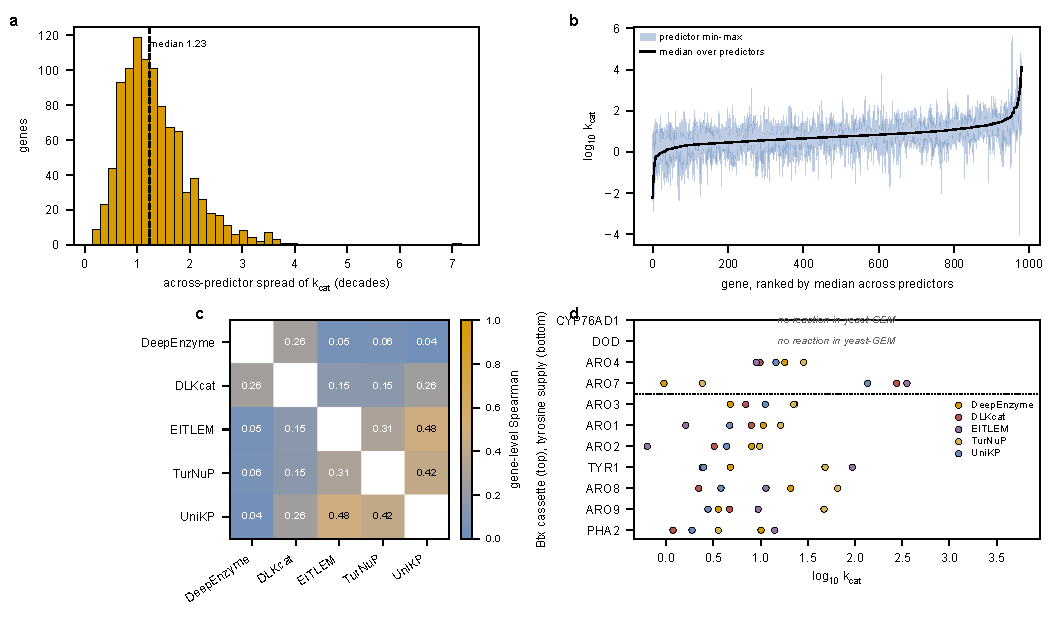
\includegraphics[width=\textwidth]{figures/per_gene_agreement_k_cat.pdf}
  \caption[Per-gene agreement between $k_{cat}$ predictors]{Agreement between the five
  $k_{cat}$ predictors at the level of a gene, over the 980 genes all five cover.
  \textbf{a}, Across-predictor spread per gene, the difference between the highest and
  lowest predictor in decades; the dashed line is the median, 1.23. \textbf{b}, The same
  spread against the dynamic range of $k_{cat}$ itself, genes ranked by their median across
  predictors: the band is the predictor min-max, the line the median. \textbf{c},
  Gene-level Spearman between predictors; the diagonal is left blank because a predictor
  against itself is 1 by construction. \textbf{d}, The genes the betaxanthin case study
  runs on. Above the dotted rule is the Btx cassette, below it the aromatic-amino-acid
  genes that supply its tyrosine precursor. \texttt{CYP76AD1} and \texttt{DOD} are
  heterologous and have no reaction in yeast-GEM, so no predictor emits a value for them.
  Generated by
  \texttt{experiments/026-metabolism-flux/scripts/plot\_per\_gene\_predictor\_agreement.py}.}
  \label{fig:per-gene}
\end{figure}

\textbf{For $k_{cat}$ the disagreement between predictors is larger than the quantity
being predicted.} The median gene moves 1.23 decades between the highest and lowest
predictor, a factor of 17, and 67 percent of genes move by more than a full decade. The
10th-to-90th-percentile range of the consensus estimate across genes is 0.94 decades. The
ratio is 1.32: choosing a different published predictor moves one gene's turnover number
further than real enzymes differ from one another. Panel b is that statement drawn, and the
band never narrows.

\textbf{For $K_M$ it is not.} The same construction over the three $K_M$ predictors gives a
median spread of 0.70 decades against a consensus range of 1.34, a ratio of 0.52, and
Boost\_KM agrees with UniKP at a gene-level Spearman of 0.75, higher than any pair of
$k_{cat}$ predictors reaches. Both facts are agreement rather than accuracy, since almost
none of these pairs has a measured value. Read that way they arrive at Wu et al.'s
conclusion from the other side: their claim is that underground metabolism separates from
known metabolism on $K_M$ rather than on $k_{cat}$, and $K_M$ is also the parameter the
instruments agree on well enough for a separation to be legible.

\textbf{The consequence for the flux layer.} An enzyme-constrained bound $v_j \le
k_{cat,j} E_j$ inherits panel a as its error bar, so a single predictor's table should not
be treated as the capacity constraint. The registry in
\texttt{torchcell/datasets/kinetics/} exists for that reason: predictor choice is a
hyperparameter with a measured effect size, not a settled detail.

%% notes-tex/026-kinetics-thermodynamics/sections/5-module.tex
%% [[torchcell.models.equivariant_cell_graph_transformer.mermaid.metabolic-module]]
%% https://github.com/Mjvolk3/torchcell/tree/main/notes-tex/026-kinetics-thermodynamics/sections/5-module.tex

\section{Where these tables enter the model\secstatus{todo}}

Figure~\ref{fig:cgt-module} places the flux module inside the cell graph transformer. The
module is neither of the two instrument classes the architecture previously had: a Type I
instrument maps a representation to a representation and a Type II instrument maps a
representation to a measured output, while the flux module maps a representation to a
\emph{flux vector}, a latent physical state from which phenotypes are then read. It sits
between them.

Three of its inputs are parameter tables rather than learned weights, and those three are
what this document builds. The $k_{cat}$ table sets the upper bound of the box that the
flux is parameterized inside, so it fixes what fluxes are reachable at all. The formation
energies set the reaction potential whose sign the second-law penalty acts on, which is
what makes that penalty a physical statement rather than a regularizer. The $K_M$ table is
built and not yet enabled, for the reason Section~\ref{sec:limits} gives.

The heterologous cassette enters as a typed perturbation on the genome-scale model, which
is what puts a betaxanthin pathway and a gene deletion inside the same object rather than
in two parallel code paths.

\tcfigfit[1.0]{figures/cgt_metabolic_module.pdf}{The cell graph transformer with the
  enzyme-constrained thermodynamic flux module. Purple marks inputs and the hash-pinned
  parameter tables built here; orange the embeddings and the Type I perturbation operators;
  red the transformer layers and the outputs; yellow the graph regularization, the
  invariant readouts and the soft constraints; blue the metabolic module, whose color slot
  was unused in the previous version of this diagram so the new content separates at a
  glance. Every hard constraint is either exact by construction, as the box and the
  capacity bound are, or relaxed to a smooth penalty; nothing is enforced by a binary
  variable, which is what makes the layer differentiable and what removes the mixed-integer
  cost a per-genotype thermodynamic program pays. The dashed $K_M$ edge marks a table that
  exists but is not yet consumed. Scaled to the text block: the source renders at 211.7 mm
  wide against a 182 mm block, so this is not shown at true print size. Source:
  \texttt{notes/torchcell.models.equivariant\_cell\_graph\_transformer.mermaid.metabolic-module.md},
  rendered by \texttt{notes/assets/publish/scripts/mermaid\_pdf.sh}.}{fig:cgt-module}

%% notes-tex/026-kinetics-thermodynamics/sections/6-limits.tex
%% [[experiments.026-metabolism-flux.kinetic-and-thermodynamic-parameter-datasets]]
%% https://github.com/Mjvolk3/torchcell/tree/main/notes-tex/026-kinetics-thermodynamics/sections/6-limits.tex

\section{What these tables cannot support\secstatus{todo}}
\label{sec:limits}

\subsection{A predicted turnover number is not a measured one\secstatus{todo}}

Every row in the $k_{cat}$ and $K_M$ builds is a model output. The tables record that in a
provenance column beside the value, because a number with no provenance becomes
indistinguishable from a measurement within two steps, and the coverage gate has to be able
to separate an experimental value, a predicted value and a filled default.

The size of the distinction is measurable. Two predictors trained on overlapping data,
applied to the same 7{,}351 pairs, disagree by a median factor of about three. Neither
model's own reported error is that large. The disagreement is the honest uncertainty on any
single value, and it is wider than any published accuracy figure would suggest, because
those figures are computed on held-out data drawn from the same corpus rather than on a
genome-scale application.

\subsection{Accuracy against the Open Enzyme Database is memorization, not generalization\secstatus{todo}}

Comparing predictions to the Open Enzyme Database looks like validation and is not. The
database aggregates BRENDA and Sabio-RK, which is what these models were trained on, so a
matched enzyme-substrate pair is almost certainly inside their training sets. Numbers from
that comparison are reported here explicitly as memorization checks.

The join also has to be on the \emph{pair}. Joining on enzyme alone compares a prediction
for one substrate against a measurement for another, and doing so moves one of these
correlations from 0.98 to 0.82 and another from 0.62 to 0.12. The looser join is the one
that is easy to write by accident.

\subsection{$K_M$ is built and deliberately not consumed\secstatus{todo}}

The flux layer does not use $K_M$. The parameter enters only through a saturation factor
$\eta_{\mathrm{sat}} = \prod_i c_i/(K_{M,i} + c_i)$, which needs intracellular metabolite
concentrations, and those are measured for 191 of 2{,}806 metabolites, 6.8 percent. Adding
$K_M$ today would add a parameter and a free variable per reaction with no anchor for
either.

The measured argument for adding it anyway is promiscuity: underground reactions show
roughly twice the $K_M$ at indistinguishable $k_{cat}$, so a $k_{cat}$-only model cannot
tell a promiscuous side activity from a native one. The measured argument against is that
the $K_M$ predictions here are the least reliable of the set, and treating them as constants
rather than as order-of-magnitude priors would put that unreliability directly into a
constraint.

\subsection{The thermodynamic gaps\secstatus{todo}}

Three, in order of how much they bind.

\textbf{Novel compounds need a licensed tool.} Adding a compound eQuilibrator has never
seen requires pKa estimates from ChemAxon's \texttt{cxcalc}. Without the license the
compound cache is read-only, so the betaxanthin intermediates that are not already in it
cannot be priced at all. This is the binding constraint on applying the method to
heterologous pathways, which is exactly where it is most wanted.

\textbf{Coverage fell.} Reaction coverage went from 77.7 percent to 42.5 percent, because a
reaction needs every participant resolved. The unresolved metabolites are dominated by
acyl-CoA isomers and combinatorial lipid species, which are chemically ordinary and merely
un-indexed under the names the model uses.

\textbf{Compartment pH is not validated.} It is implemented, it produces shifts too large
to believe, and the pH table is assumed rather than sourced. Until that is diagnosed the
uniform build is the one to use, which means transport thermodynamics is set to zero by
construction and the proton motive force is absent from the model.

\subsection{What the mirror records when a predictor cannot run\secstatus{todo}}

All six now run. Where a predictor could not be run at all, the mirror records
\texttt{runnable: false} with the specific blocker, so that a gap in coverage is never
mistaken for a modeling choice.

Boost\_KM carried that flag until its weights were read rather than its filenames, and the
correction is recorded in Section~\ref{sec:mirrors} rather than quietly dropped: the
repository does ship fitted regressors, and the obstacle was never a missing model. It was
that UniRep is a TensorFlow~1 mLSTM stepping one residue at a time on CPU, which on a first
attempt occupied roughly 85 cores. The ESM-1b variant Wu et al. actually used replaces that
stage with a transformer that embeds all 887 enzymes on one GPU in four minutes.

%% notes-tex/026-kinetics-thermodynamics/sections/7-sources.tex
%% [[experiments.026-metabolism-flux.kinetic-and-thermodynamic-parameter-datasets]]
%% https://github.com/Mjvolk3/torchcell/tree/main/notes-tex/026-kinetics-thermodynamics/sections/7-sources.tex

\section{Every source, for citation and for the mirror\secstatus{todo}}
\label{sec:sources}

Each predictor is a published method, a code repository at a pinned commit, and a weights
archive, and the three are cited differently. The tables below carry all of them so a
reference can be added to the library and a manifest field filled without re-deriving the
provenance. Every commit and \texttt{sha256} comes from
\texttt{\$DATA\_ROOT/models/kinetics/<name>/manifest.json} or from
\texttt{mirror\_kinetic\_models.py}; the DOIs were verified against Crossref rather than
recalled.

\subsection{Papers\secstatus{todo}}

\begin{table}[H]
  \centering
  \footnotesize
  \caption[Papers to cite]{The publication behind each artifact used in this document.}
  \label{tab:papers}
  %% SOURCE: manifest.json per mirror + Crossref verification; see notes for the audit.
  \begin{tabular}{@{}p{0.15\textwidth}p{0.46\textwidth}p{0.31\textwidth}@{}}
    \hline
    Tool & Paper & DOI \\
    \hline
    DLKcat & Li et al., Deep learning-based $k_{cat}$ prediction enables improved
      enzyme-constrained model reconstruction. \emph{Nat Catal} 5:662--672, 2022
      & \texttt{10.1038/s41929-022-00798-z} \\
    UniKP & Yu et al., UniKP: a unified framework for the prediction of enzyme kinetic
      parameters. \emph{Nat Commun} 14:8211, 2023
      & \texttt{10.1038/s41467-023-44113-1} \\
    EITLEM & Shen et al., EITLEM-Kinetics: a deep-learning framework for kinetic parameter
      prediction of mutant enzymes. \emph{Chem Catal} 4:101094, 2024
      & \texttt{10.1016/j.checat.2024.101094} \\
    TurNuP & Kroll et al., Turnover number predictions for kinetically uncharacterized
      enzymes using machine and deep learning. \emph{Nat Commun} 14:4139, 2023
      & \texttt{10.1038/s41467-023-39840-4} \\
    DeepEnzyme & Wang et al., DeepEnzyme: a robust deep learning model for improved enzyme
      turnover number prediction. \emph{Brief Bioinform} 25(5):bbae409, 2024
      & \texttt{10.1093/bib/bbae409} \\
    Boost\_KM & Kroll et al., Deep learning allows genome-scale prediction of Michaelis
      constants from structural features. \emph{PLoS Biol} 19:e3001402, 2021
      & \texttt{10.1371/journal.pbio.3001402} \\
    eQuilibrator & Beber et al., eQuilibrator 3.0: a database solution for thermodynamic
      constant estimation. \emph{Nucleic Acids Res} 50:D603--D609, 2022
      & \texttt{10.1093/nar/gkab1106} \\
    Component contribution & Noor et al., Consistent estimation of Gibbs energy using
      component contributions. \emph{PLoS Comput Biol} 9:e1003098, 2013
      & \texttt{10.1371/journal.pcbi.1003098} \\
    Yeast-MetaTwin & Wu et al., Systematically exploring yeast metabolism through
      retrobiosynthesis and deep learning. \emph{Nat Catal} 9:434--447, 2026
      & \texttt{10.1038/s41929-026-01523-w} \\
    \hline
  \end{tabular}
\end{table}

\subsection{Code and weights\secstatus{todo}}

\begin{table}[H]
  \centering
  \footnotesize
  \caption[Code repositories and weight archives]{What was mirrored, at which revision.
  A commit is given in full because a short hash is not a pin.}
  \label{tab:code}
  %% SOURCE: $DATA_ROOT/models/kinetics/<name>/manifest.json (per-file sha256 + revision).
  \begin{tabular}{@{}p{0.14\textwidth}p{0.40\textwidth}p{0.38\textwidth}@{}}
    \hline
    Tool & Repository, at commit & Weights \\
    \hline
    DLKcat & \texttt{SysBioChalmers/DLKcat} \newline
      \texttt{7c15d0d4a7ac029f9d75564d9f2a93874aeaaec7} & in repo, extensionless
      \texttt{state\_dict} \\
    UniKP & \texttt{Luo-SynBioLab/UniKP} \newline
      \texttt{3ad5576aaa2c8c0dd0e0b6c283c1d365ab23c6ea} &
      HuggingFace \texttt{HanselYu/UniKP} \\
    EITLEM & \texttt{XvesS/EITLEM-Kinetics} \newline
      \texttt{7bb9d6668d86263f17dddc1915fccff5712fd511} &
      Zenodo \texttt{10.5281/zenodo.16153803}, 12.3 GB \\
    TurNuP & \texttt{AlexanderKroll/kcat\_prediction} \newline
      \texttt{98d88a37b66f64381086b5492f315e763c528fa0} &
      Zenodo \texttt{10.5281/zenodo.8367052} and
      \texttt{10.5281/zenodo.8038678} \\
    DeepEnzyme & \texttt{hongzhonglu/DeepEnzyme} \newline
      \texttt{d225ec31a1079177eea38fcf44c5c4b7afe516d8} &
      figshare \texttt{10.6084/m9.figshare.25771062.v2} \\
    Boost\_KM & \texttt{AlexanderKroll/KM\_prediction} \newline
      \texttt{432a4fc02afa20fcb8296fb96ce035a99ae33e85} &
      in repo; the ESM-1b variant is vendored in the Yeast-MetaTwin release \\
    ESM-1b & Meta \texttt{fair-esm}, base checkpoint &
      \texttt{esm1b\_t33\_650M\_UR50S.pt}, sha256 \texttt{0569754e\ldots83a8b1} \\
    Yeast-MetaTwin & \texttt{LiLabTsinghua/Yeast-MetaTwin} \newline
      \texttt{de1268eea271a67ffb0581aab51b3549c8020950} &
      Zenodo \texttt{10.5281/zenodo.13911783}, 6.6 GB \\
    \hline
  \end{tabular}
\end{table}

\subsection{Four provenance defects to repair\secstatus{todo}}

These are recorded rather than fixed silently, because each one breaks the rebuild
guarantee in a different way.

\begin{itemize}\setlength{\itemsep}{2pt}
  \item \textbf{EITLEM's recorded source URL is dead.} The manifest holds
    \texttt{XvQiao/EITLEM-Kinetics}, which now returns 404; the repository was renamed to
    \texttt{XvesS/EITLEM-Kinetics}. The pinned commit still resolves there, so the mirrored
    bytes are fine and only the retrieval command needs updating.
  \item \textbf{DeepEnzyme's retrieval command is a placeholder.} It contains the literal
    text \texttt{<figshare 10.6084/m9.figshare.25771062.v2>} rather than a URL, so that one
    file cannot be re-fetched by running the record.
  \item \textbf{eQuilibrator and Yeast-MetaTwin have no manifest.} Both sit outside
    \texttt{models/kinetics/}. The MetaTwin commit had to be read out of \texttt{.git}, and
    \texttt{metatwin.rar} is pinned by size alone with no \texttt{sha256}.
  \item \textbf{All six kinetics manifests carry \texttt{citation\_key: null}.} Once these
    papers are in the mirror, that field joins each weight file to its publication, which is
    what makes a predicted value citable rather than merely traceable.
\end{itemize}

One extraction hazard is worth recording alongside them. \texttt{bsdtar} reading
\texttt{esm1b\_t33\_650M\_UR50S.pt} out of the 6.6 GB RAR \textbf{exited 0 and wrote
649{,}783{,}100 bytes} where the archive's own listing says 7{,}828{,}576{,}466. The
truncation is silent, and a checkpoint that short still opens far enough to look like a
file. It was caught by comparing against the listed size and then confirmed by
\texttt{torch.load} refusing it. The bytes finally used were fetched from the published
\texttt{fair-esm} URL and verified to the recorded \texttt{sha256}, which is the general
lesson: a size or hash check is what makes an extractor's exit code mean anything.


\end{document}
